\section{Interfejs użytkownika}
    \tab Oprogramowanie pozwala na komunikację z „Azorem” oraz reprezentację danych pomiarowych.

    % Po uruchomieniu programu należy z wiersza poleceń wybrać port szeregowy, wykorzystywany do komunikacji przez moduł Bluetooth.
    

    \subsection{Podstawowe sterowanie „Azorem”}
        \tab Podstawowym sposobem sterowania jest interfejs graficzny, który można podzielić na 3 części:

        \subsubsection{Mapa skanowanego obszaru}        
            \tab Największą część okna aplikacji zajmuje mapa skanowanego obszaru, 
            na której czerwonymi liniami zaznaczone są przeszkody a niebieska strzałka reprezentuje „Azora”.

        \subsubsection{Radar}
            \tab Poniżej mapy po lewej stronie znajduje się radar. 
            Którego klikniecie wywołuje funkcję zbierania informacji na temat tego co widzi „Azor” oraz narysowanie ich na mapie. 
            Dodatkowo, na radarze widać aktualną pozycję „głowy Azora”.
        
        \subsubsection{Przyciski sterujące}
            \tab Ostatnią ale nie mniej ważną częścią interfejsu jest 6 strzałek i kulka. 
            Dzięki strzałkom góra/dół można poruszać „Azorem” w przód i w tył.
            Dwie kolejne strzałki w prawo i lewo pozwalają na obrót „Azora” o $90^\circ$.
            Ostatnie dwie strzałeczki odpowiadają za obrót głowy o $15^\circ$, a kuleczka pośrodku odpowiada za wykonanie pojedynczego pomiaru odległości.

    \begin{figure}[!ht]
        \centering
        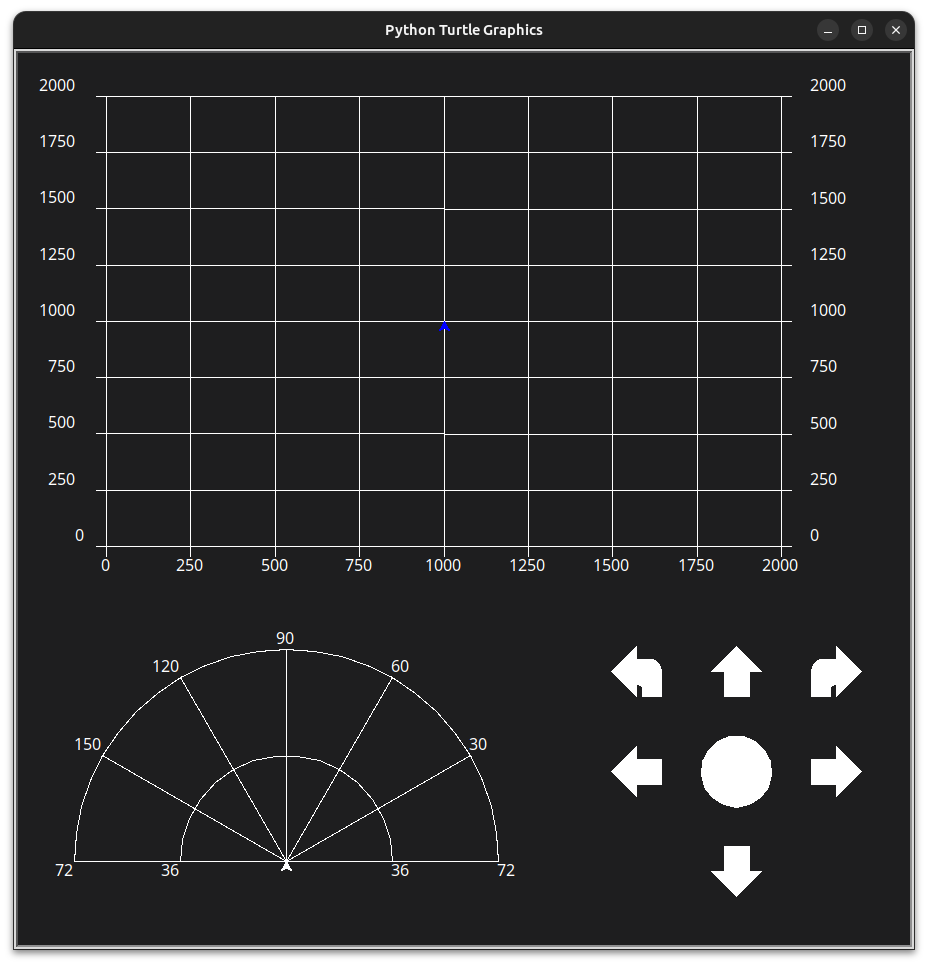
\includegraphics[height = 0.43\textheight]{Img/GUI.png}
        \caption{Interfejs graficzny}
    \end{figure}
        
    
    \newpage
    \subsection{Zaawansowane sterowanie}
        \tab Oprócz sterowania za pomocą przycisków istnieje możliwość wysyłania poleceń do „Azora” za pośrednictwem Command Line'a.
        \begin{figure}[!h]
            \centering
            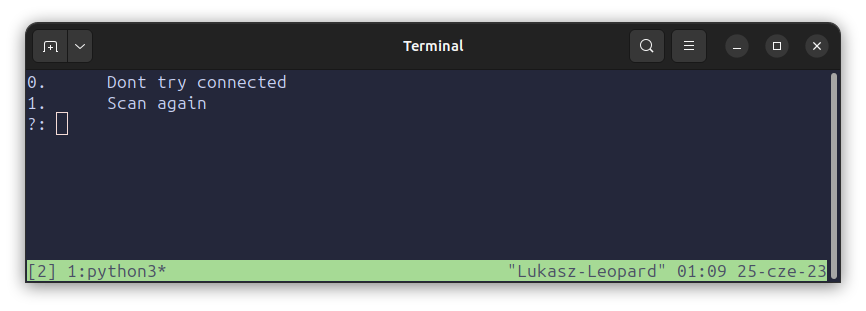
\includegraphics[width = 0.8\textwidth]{Img/CLI.png}
            \caption{Wybór portu do sterowania}
        \end{figure}
        \\Możliwe komendy:
        \begin{itemize}
            \item \textit{forward [wartość]}            - przemieszczenie „Azora” w przód o podaną odległość w mm, domyślna wartość to 100 mm,
            \item \textit{backward [wartość]}           - przemieszczenie „Azora” w tył o podaną odległość w mm, domyślna wartość to 100 mm,
            \item \textit{left [wartość]}               - obrót „Azora” w lewo o podany kąt, wartość domyślna to $90^\circ$,
            \item \textit{right [wartość]}              - obrót „Azora” w prawo o podany kąt, wartość domyślna to $90^\circ$,
            \item \textit{head left/right [wartość]}    - obrót czujnikiem odległości w lewo/prawo o podany kąt,wartość domyślna to $6^\circ$,
            \item \textit{head set [wartość]}           - obrót „głową Azora” do zadanego kąta z zakresu $0^\circ-180^\circ$, domyślnie $90^\circ$, co oznacza „patrzenie” w przód,
            \item \textit{head measure}                 - wykonanie pomiaru odległości dla obecnego ustawienia czujnika odległości,
            \item \textit{acc}                          - zwrócenie aktualnej wartości przyspieszenia na każdej z 3 osi,
            \item \textit{magnet}                       - zwrócenie zmierzonej wartości pola magnetycznego na każdej z 3 osi,
            \item \textit{azimuth}                      - zwrócenie aktualnej wartości azymutu,
            \item \textit{distance}                     - zwrócenie wartości ostatnio pokonanej odległości,
            \item \textit{time}                         - zwrócenie czasu pracy silników,
            \item \textit{velocity}                     - zwrócenie wartości ostatnio zarejestrowanej prędkości,
            \item \textit{radar}                        - wykonanie automatycznego pomiaru odległości w zakresie $0^\circ-180^\circ$ z krokiem $3^\circ$,
            \item \textit{clear}                        - czyszczenie mapy,
            \item \textit{exit}                         - zakończenie działania programu,
        \end{itemize}
    